\documentclass{beamer}
\usepackage{graphicx, float, movie15, hyperref}

\begin{document}
\title{Visualizing Multi-View Stereo}
\author{Andrew Moran, Ben Eysenbach}
\date{December 9, 2014}

\frame{\titlepage}

\section{Introduction}

\begin{frame}{Motivation}
  Pipelines are hard to construct.
  
  \begin{center}
  \begin{tabular}{ccccc}
    & & Algorithm, & & \\ 
    & & Parameters & & \\ 
    & & $\downarrow$ & &  \\ 
    Input & $\rightarrow$ & $\blacksquare$ & $\rightarrow$ & Output \\ 
  \end{tabular} 
  \end{center}
  
\end{frame}

\begin{frame}{Motivation}
  Better:
  
  \begin{center}
    \begin{tabular}{ccccccccc}
      & & Algorithm, & & & & Algorithm, & & \\ 
      & & Parameters & & & & Parameters & & \\ 
      & & $\downarrow$ & & & & $\downarrow$ & & \\ 
      Input & $\rightarrow$ & $\blacksquare$ & $\rightarrow$ & ... & $\rightarrow$ & $\blacksquare$ & $\rightarrow$ & Output \\ 
    \end{tabular} 
  \end{center}

\end{frame}

\begin{frame}{Evaluating each Step}
  How to evaluate the output of each step?\\
  
  Quantitative:
  \begin{itemize}
    \item Great if ground truth is known
    \item Harder if you need to construct an error function
    \item Algorithms can fail in different ways
  \end{itemize}
  
  Qualitative:
  \begin{itemize}
    \item Great for debugging and comparing output
    \item Great for 2D operations
    \item Hard for 3D operations
  \end{itemize}
  
\end{frame}  
  
\section{Feature Matching}

\begin{frame}{Feature Matching}

  \centering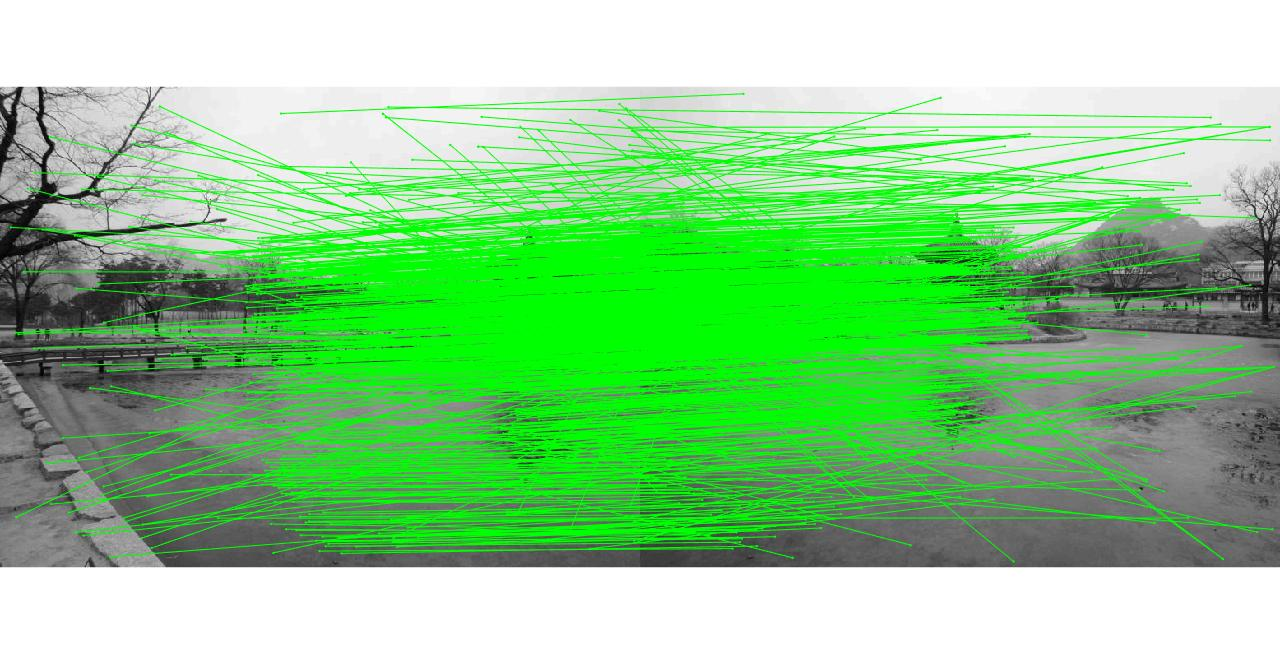
\includegraphics[height=.4\textheight]{Images/sift.jpg}

  \begin{centering}
  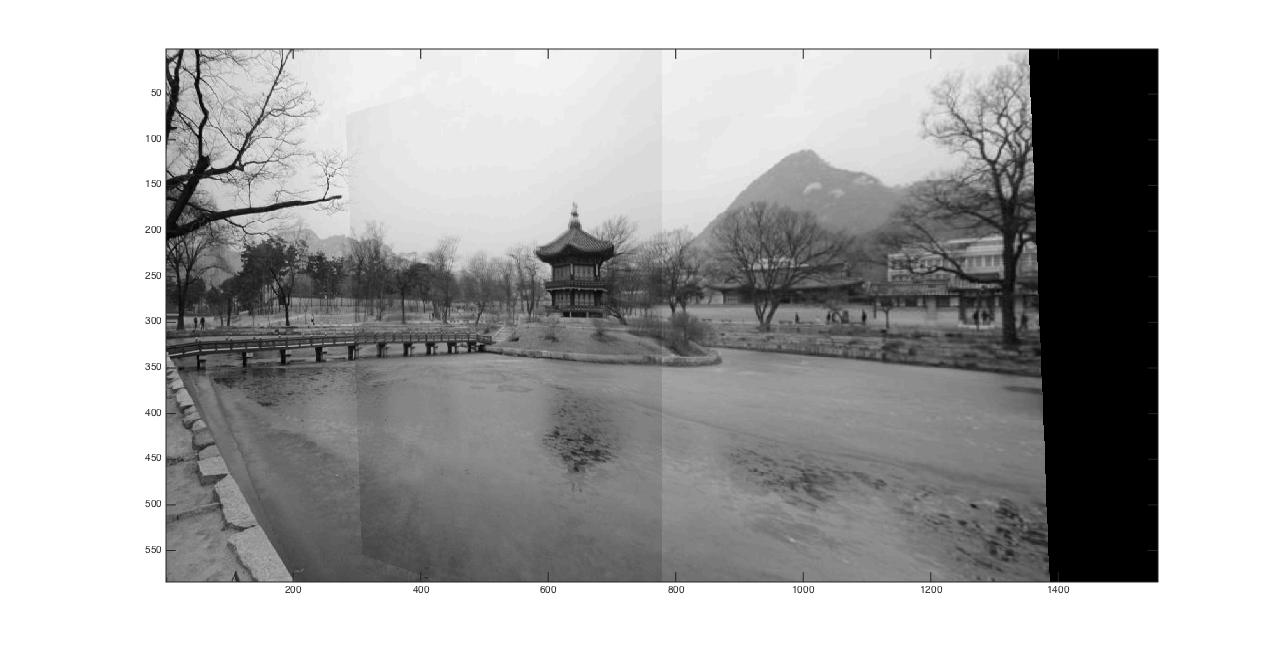
\includegraphics[height=.4\textheight]{Images/panorama.jpg}
  \end{centering}
\end{frame}

\begin{frame}{Point Cloud}
  \begin{columns}
    \column{.5\textwidth}
    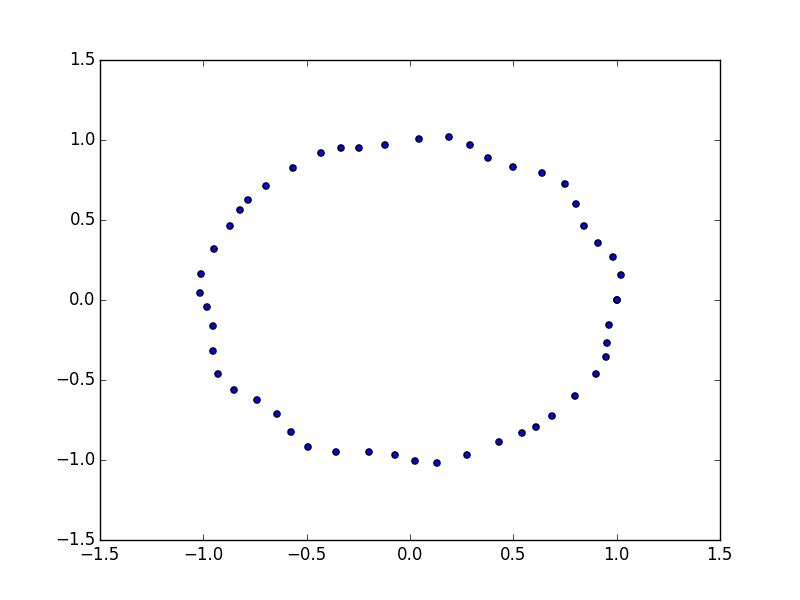
\includegraphics[width=\textwidth]{Images/point_cloud.png}
    \column{.5\textwidth}
    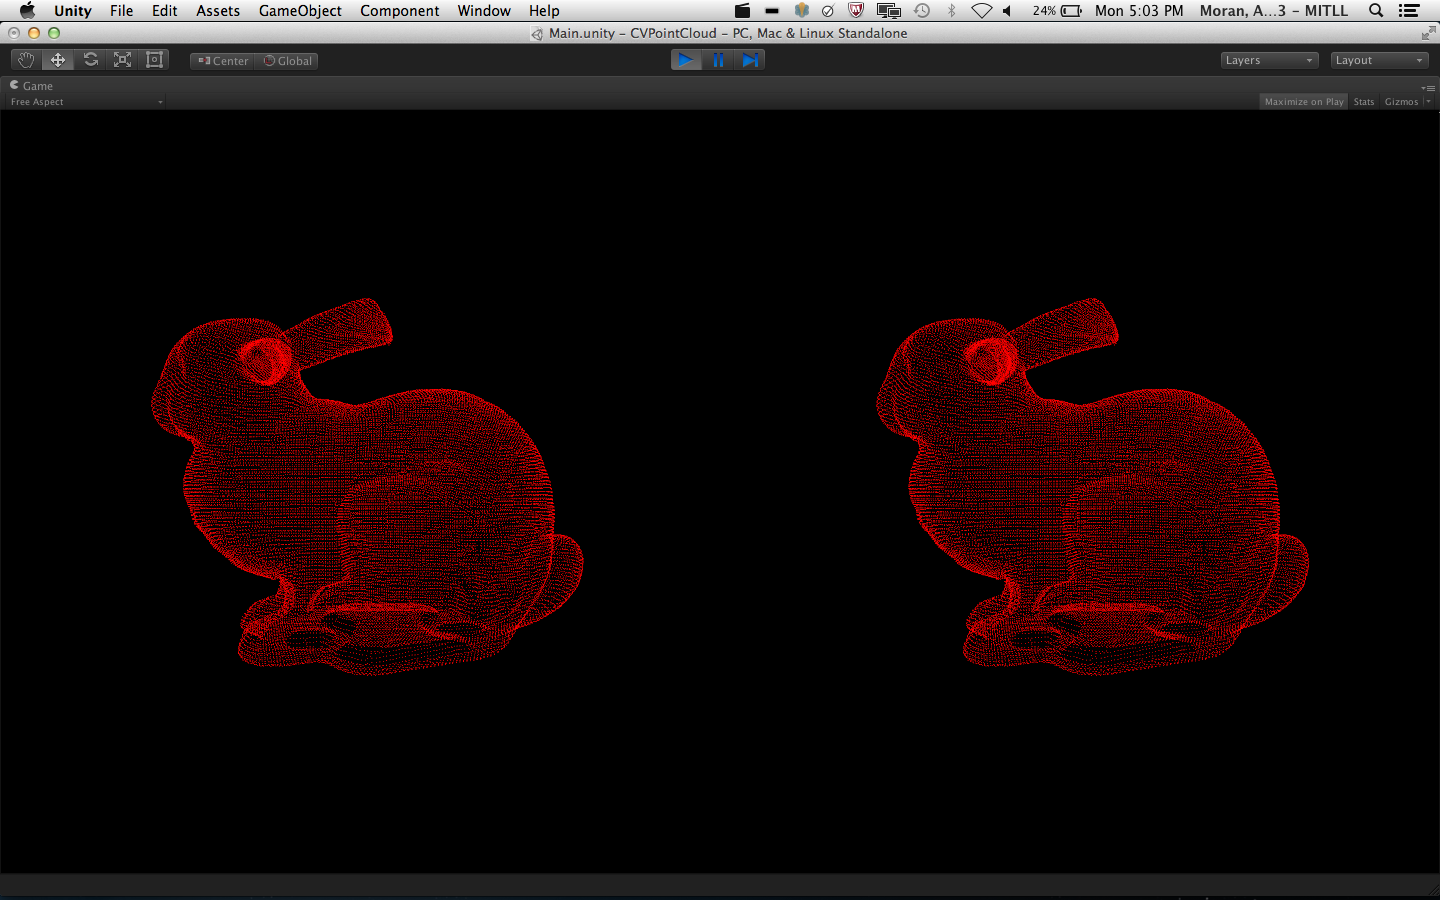
\includegraphics[width=\textwidth]{Images/bunny_dense.png}
  \end{columns}
\end{frame}

\begin{frame}{Normal Estimation}
  \begin{columns}
    \column{.5\textwidth}
  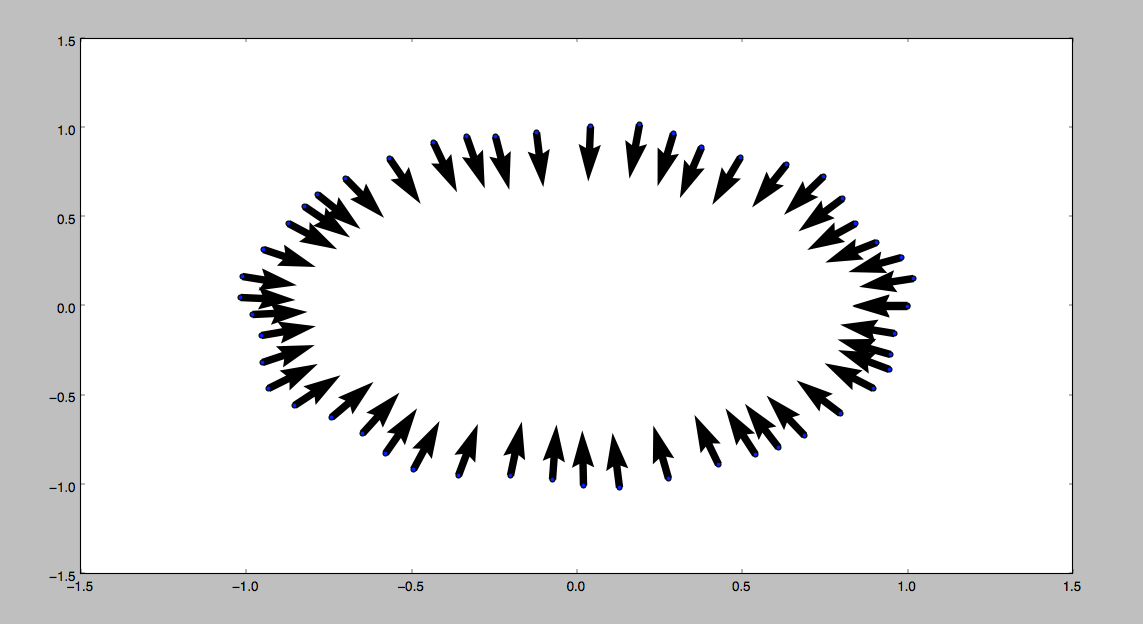
\includegraphics[width=\textwidth]{Images/normals.png}
    \column{.5\textwidth}
    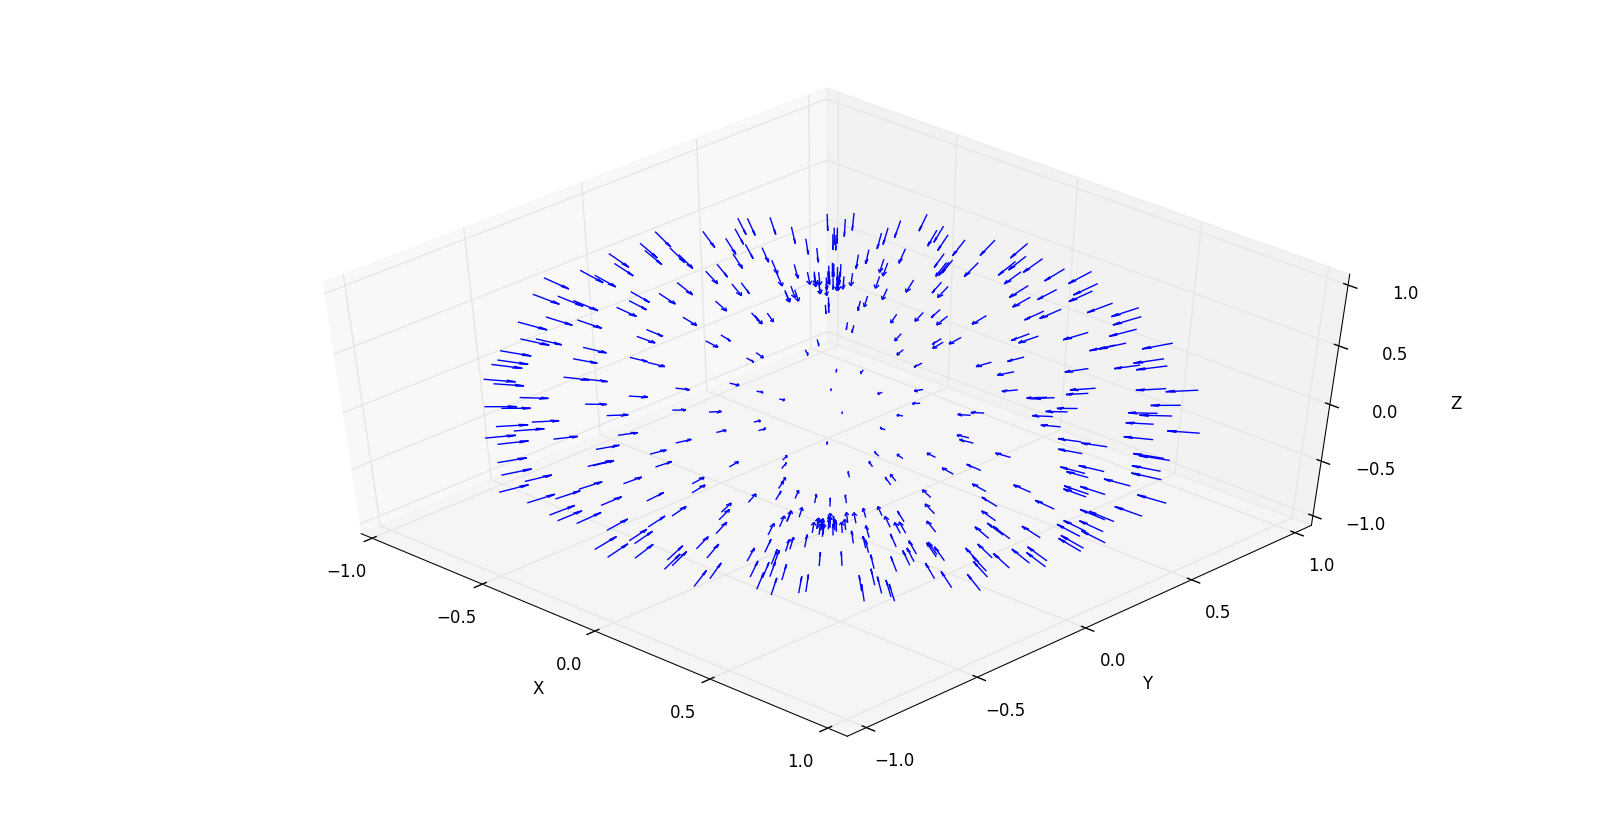
\includegraphics[width=\textwidth]{Images/3d_normals.png}
  \end{columns}
  
\end{frame}

\begin{frame}{Spatial Data Structures}
    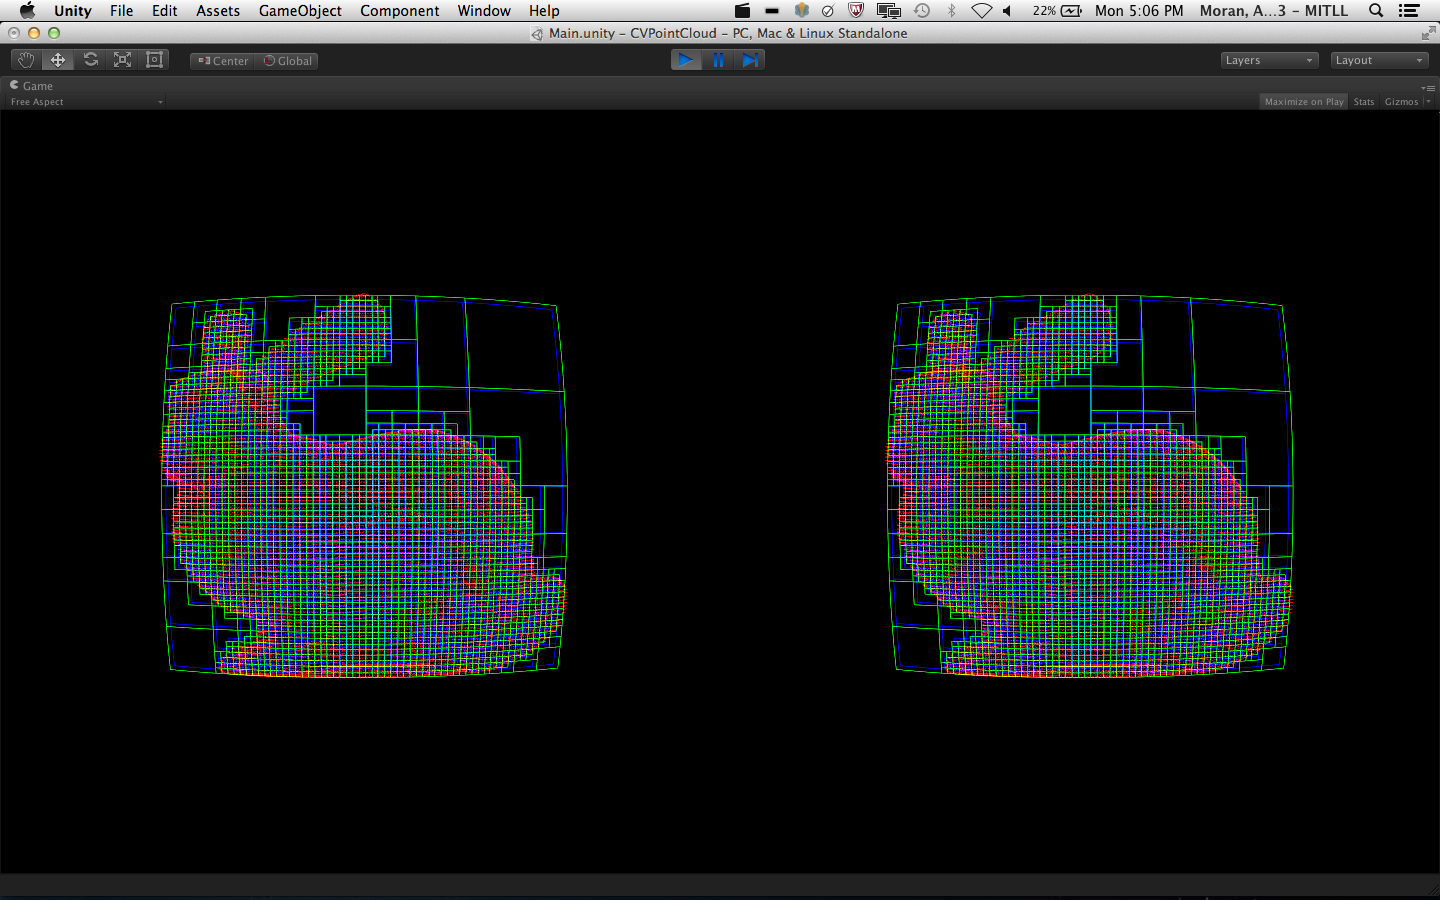
\includegraphics[width=\textwidth]{Images/bunny_ortho_octree6.png}
\end{frame}

\begin{frame}{Spatial Data Structures}
    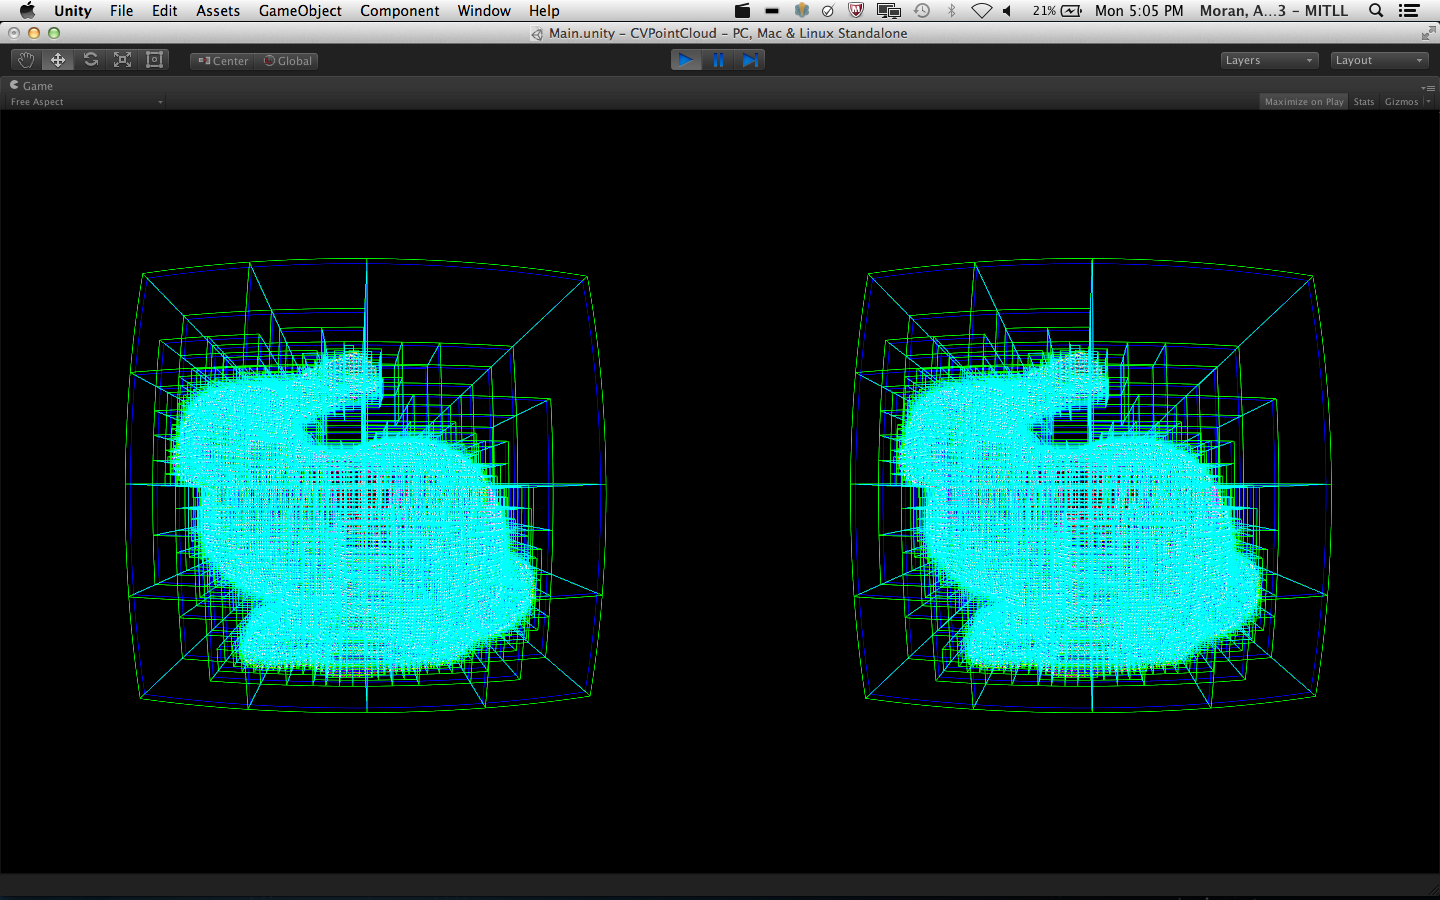
\includegraphics[width=\textwidth]{Images/bunny_front_octree6.png}
\end{frame}


\begin{frame}{Marching Cubes}
  \begin{columns}
    \column{.5\textwidth}
    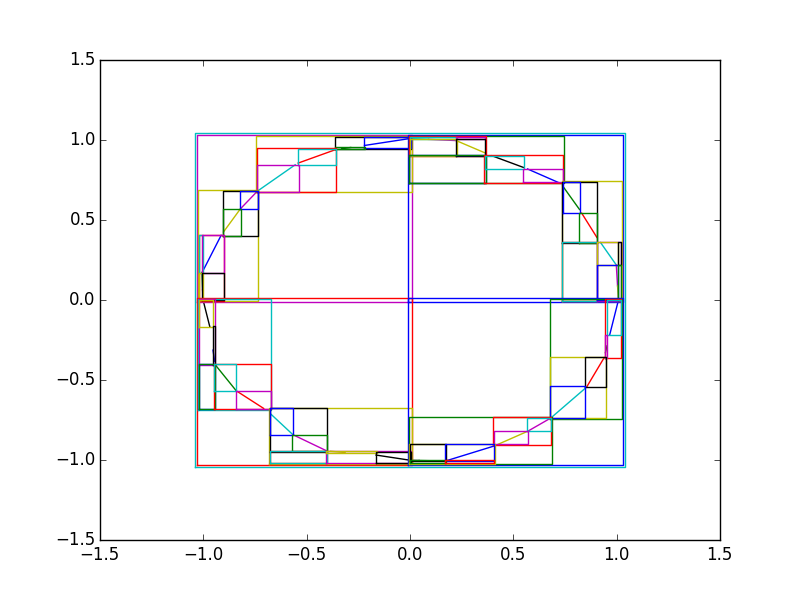
\includegraphics[width=\textwidth]{Images/marching_squares.png}
    \column{.5\textwidth}
    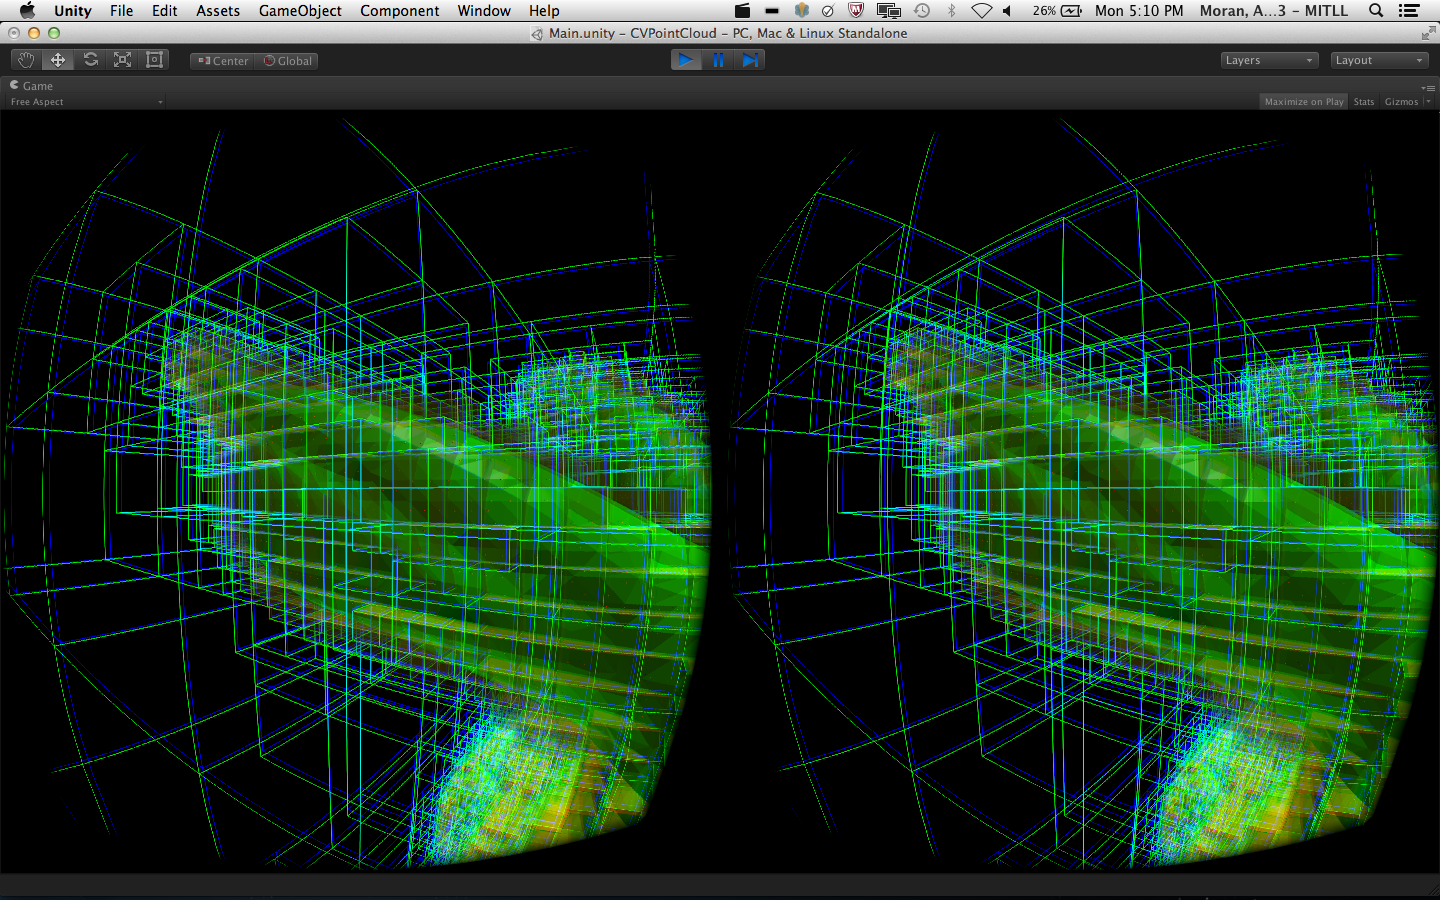
\includegraphics[width=\textwidth]{Images/bunny_ear_octreeCubesMesh.png}
  \end{columns}
\end{frame}

\begin{frame}{Surface Reconstruction}
  \begin{columns}
    \column{.5\textwidth}
    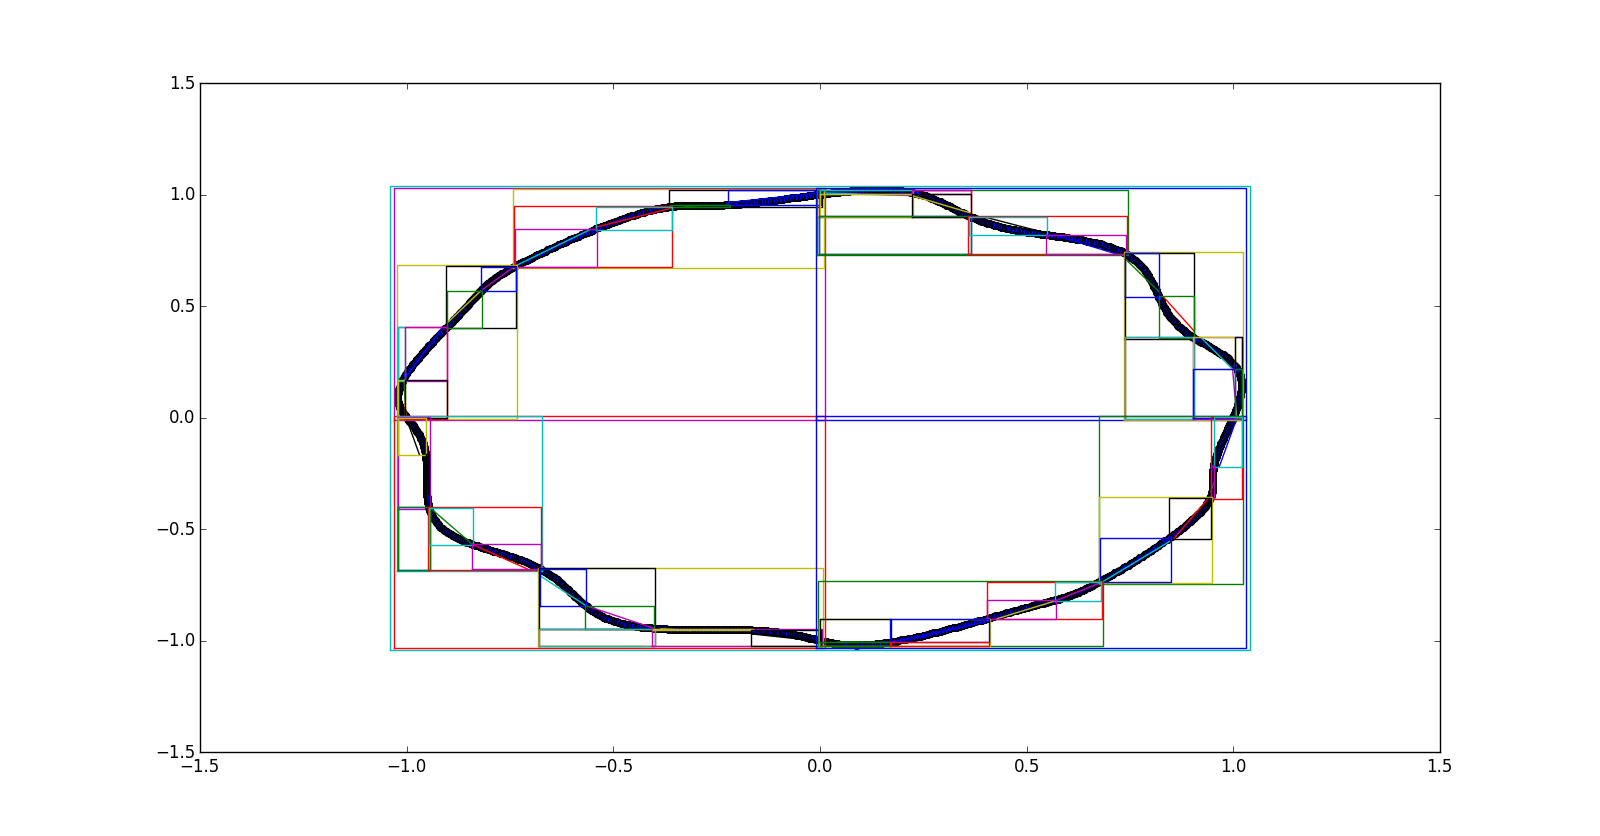
\includegraphics[width=\textwidth]{Images/quadtree.png}
    \column{.5\textwidth}
    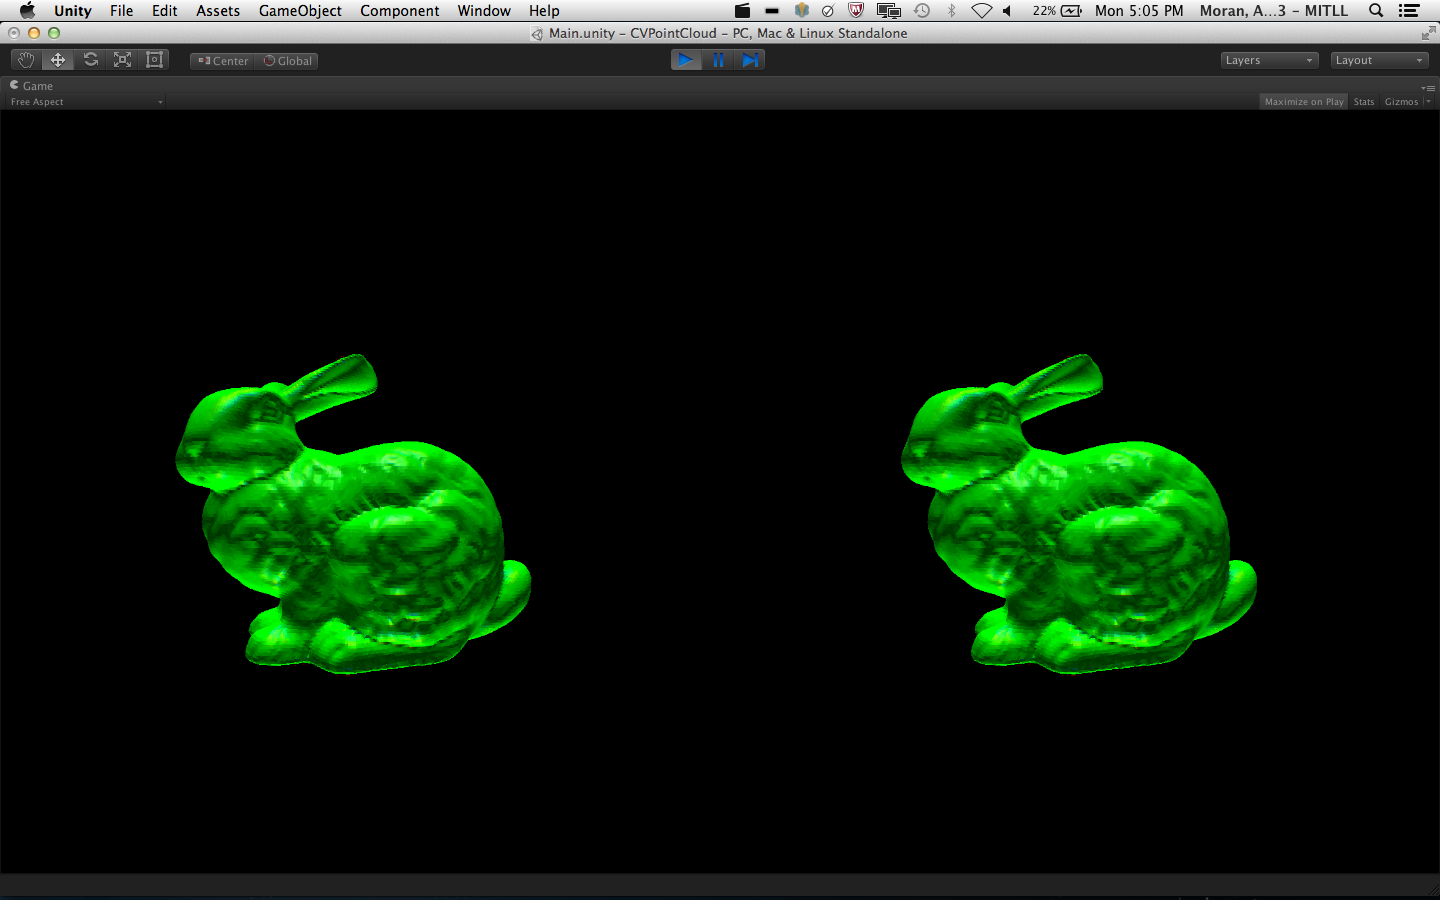
\includegraphics[width=\textwidth]{Images/bunny_front_meshReg.png}
  \end{columns}
\end{frame}


\begin{frame}{Results}
  % screenshot
  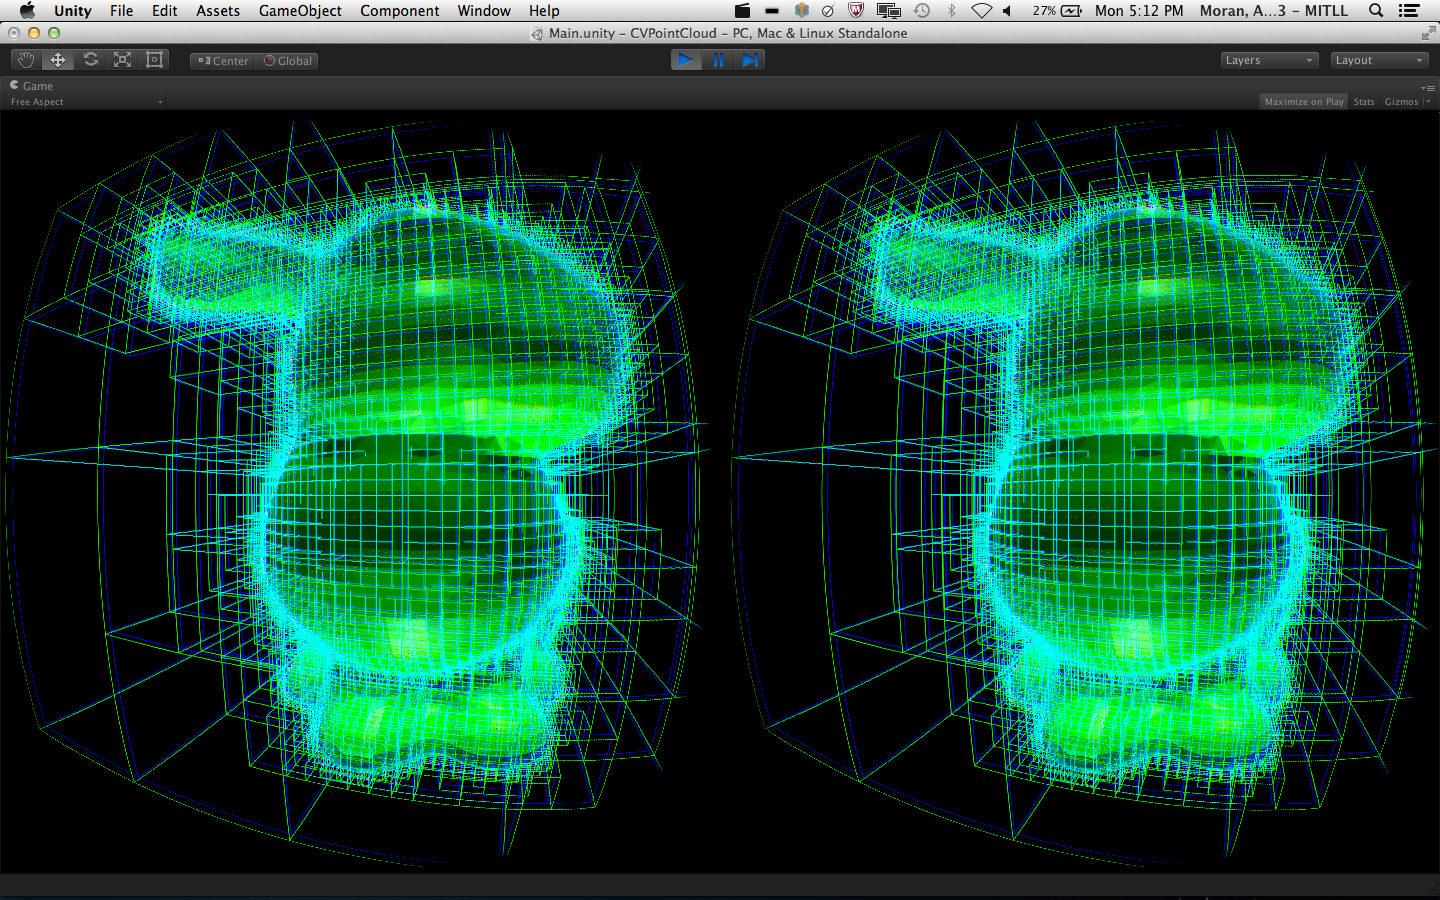
\includegraphics[width=\textwidth]{Images/bunny_side_meshOctree.png}
  
  \url{http://google.com}
\end{frame}

\begin{frame}{Thank You}
    % cool picture
\end{frame}

\begin{frame}{Questions?}
\end{frame}
  
\end{document}